
\documentclass[12pt,A4paper,titlepage]{article}

%PAQUETES
\usepackage[spanish]{babel}
\usepackage[utf8]{inputenc} %Este paquete permite poner acentos directamente y ees
\usepackage{fontenc}
\usepackage{amsmath}
\usepackage{graphicx}%[pdftex]
\usepackage{graphicx, wrapfig}
\usepackage{fancyhdr}
\usepackage{anysize}
\usepackage{verbatim}
\usepackage{enumitem}
\usepackage{advdate}
\usepackage{colortbl}
\usepackage{amsmath}
\usepackage{hyperref}
\usepackage{amssymb}
\usepackage[dvips,final]{epsfig}
\usepackage{epstopdf}
\usepackage{enumitem}
\marginsize {2.5cm}{2.5cm}{2.5cm}{2.5cm} %Primero margen izquierdo, Segundo margen derecho, Tercero margen superior, Cuarto margen inferior.

%Línea de presentación
\usepackage{fancyhdr}
\pagestyle{fancy}
\fancyhf{}
\fancyhead[L]{Síntesis de Redes Activas - Trabajo Práctico 4}
\fancyfoot[LE,RO]{\thepage}
\fancyfoot[LO]{Armida - Ruiz Tatur}
\renewcommand{\footrulewidth}{0.1pt}

%CARATULA
\begin{document}

\begin{titlepage}

\thispagestyle{empty}



\begin{center}
    
\includegraphics[scale=0.4]{Imagenes/unc_logo.png}
    
\includegraphics[scale=0.4]{Imagenes/fcefyn_logo.jpg}
    \\[1cm]
    \vspace{5pt}
    \LARGE \textbf{Universidad Nacional de Córdoba}\\[0.5cm] 
    \large \textbf{Facultad de Ciencias Exactas, Físicas y Naturales} \\[0.5cm] 
    \large \textbf{Síntesis de Redes Activas - Trabajo Práctico 4}
    \\[0.5cm]
    \large Diseño de amplificadores utilizando VFA y CFA
    \\[0.2cm] 
    \vspace{60pt}
    \begin{table}[!h]
    \centering
    \begin{tabular}{ll}
    \multicolumn{1}{c}{Nombre} & \multicolumn{1}{c}{DNI} \\
    Armida Abril & 41.436.299 \\
    Ruiz Tatur Manuel & 40.963.553
    \end{tabular}
    \end{table}
    \vspace{20pt}
    \begin{table}[!h]
    \centering
    \begin{tabular}{ll}
    \multicolumn{1}{c}{Docentes} & Ing. Ferreyra Pablo \\ & Ing. César Reale \\
    \end{tabular}
    \end{table}
    \vspace{20pt}
    \large 2023
\end{center}

\end{titlepage}

\newpage
\tableofcontents %Arma el índice
    %%Despues cambiar el nombre

\newpage

\section{Objetivos}
\hspace{1mm} Se pretende diseñar amplificadores utilizando tecnologías VFA (Amplificador Realimentado por Tensión) y CFA (Amplificador Realimentado por Corriente) aplicando conceptos de compensación.

\bigskip
\hspace{1mm} Se analizarán tres circuitos amplificadores compuestos a partir de las tecnologías nombradas en el párrafo anterior. El primer circuito está conformado por dos VFA, en tanto que el segundo y tercer circuito estarán compuestos por un CFA y un VFA. El esquema de estos tres circuitos es el mismo y se presenta a continuación.

\begin{figure}[!h]
    \centering
    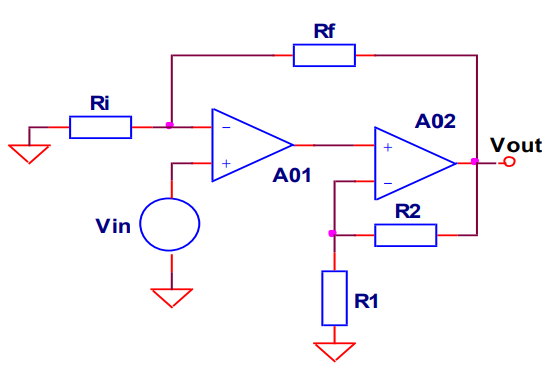
\includegraphics[scale=0.7]{Objetivos.png}
    \caption{Esquema del amplificador compuesto}
\end{figure}

\hspace{1mm} En el armado de los circuitos, los integrados utilizados para los VFA serán los LM324 de dos polos y, para el CFA será el LM6181 cuya transimpedancia también tiene dos polos. 

\bigskip
\hspace{1mm} Los requerimientos para dichos circuitos amplificadores son los expuestos seguidamente.
\begin{itemize}[itemsep=1pt]
    \item Ganancia global: \(A_{vf} = 20~dB\)
    \item Máxima planicidad de módulo: \(M_{\phi}=65°\) o \(Q_p=0.707\)
\end{itemize}

\newpage
\section{Consigna}
\subsection{Circuito I: VFA-VFA}
\hspace{1mm} Empleando la tecnología VFA y el circuito integrado LM324, proceder a realizar las siguientes consignas.
\begin{enumerate}[itemsep=1pt, label=\alph*.] 
    \item Diseñar el amplificador compuesto VFA+VFA.
    \item Calcular el ancho de banda potencial, la frecuencia del polo de la función de transferencia a lazo cerrado y el ancho de banda a \(-3~dB\).
     \item Medir el ancho de banda a \(-3~dB\).
     \item Estimar el margen de fase obtenido en base a la respuesta al escalón del amplificador compuesto.
\end{enumerate}

\subsection{Circuito II: VFA-CFA}
\hspace{1mm} Utilizando las tecnologías VFA y CFA, así como los circuitos integrados LM324 y LM6181, proporcionar respuesta a los siguientes apartados.
\begin{enumerate}[itemsep = 1pt, label=\alph*.]
    \item Diseñar el amplificador compuesto VFA+CFA para máxima planicidad de módulo y que además cumpla con un ancho de banda potencial aproximado de \(f_g=2~MHz\). Tener en cuenta la presencia del segundo polo del VFA.
    \item Calcular el ancho de banda potencial, la frecuencia del polo de la función de transferencia a lazo cerrado y el ancho de banda a \(-3~dB\).
    \item Medir el ancho de banda a \(-3~dB\).
    \item Estimar el margen de fase obtenido en base a la respuesta al escalón del amplificador compuesto.
\end{enumerate}

\subsection{Circuito III: VFA-CFA}
\hspace{1mm} Insertar en la configuración anterior una red de compensación \textbf{cero-polo} (a la salida del VFA) de tal modo que el cero de la red cancele el segundo polo del VFA. Ubicar el polo de la red a una octava de su cero. Retocar la ganancia del CFA realimentado para compensar la atenuación introducida por la red. Constatar la \textbf{mejora del margen de fase} a través de la respuesta escalón. 

\hspace{1mm} Seguidamente, realizar las siguientes consignas.
\begin{enumerate}[label=\alph*.]
    \item Calcular y medir el margen de fase, el ancho de banda potencial, la frecuencia del polo de la función de transferencia a lazo cerrado y el ancho de banda a \(-3~dB\).
    \item Calcular el ancho de banda potencial, la frecuencia del polo de la función de transferencia a lazo cerrado y el ancho de banda a \(-3~dB\).
    \item Medir el ancho de banda a \(-3~dB\).
    \item Estimar el margen de fase obtenido en base a la respuesta al escalón del amplificador compuesto.
\end{enumerate}

\newpage
\section{Marco teórico}

\subsection{Amplificador Realimentado por Tensión (VFA)}

\hspace{1mm} Un amplificador VFA (Voltage Feedback Amplifier, por sus siglas en inglés) es un tipo de amplificador electrónico que se utiliza para amplificar señales eléctricas, como señales de voltaje, corriente o potencia. La característica principal de un amplificador VFA es que su ganancia y comportamiento de amplificación están determinados principalmente por la retroalimentación de voltaje.

\bigskip 
\hspace{1mm} En un amplificador VFA, una parte de la señal de salida se toma y se compara con la señal de entrada original utilizando realimentación negativa. La diferencia entre estas dos señales se utiliza para generar una señal de error que se amplifica y luego se utiliza para corregir la señal de salida, manteniendo la amplificación dentro de los límites deseados y estables.

\bigskip 
\hspace{1mm} La ganancia y las características del amplificador VFA están controladas por los componentes pasivos y activos utilizados en su diseño.

\bigskip
\begin{figure}[!h]
    \centering
    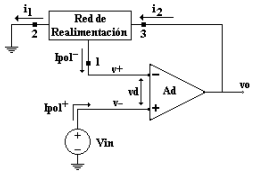
\includegraphics[scale=1]{Imagenes/VFA.png}
    \caption{VFA}
\end{figure}

\bigskip
\hspace{1mm} Este amplificador se representa interiormente por el siguiente modelo.

\bigskip
\begin{figure}[!h]
    \centering
    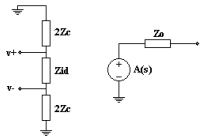
\includegraphics[scale=1]{Imagenes/VFA Modelo de amplificador real.png}
    \caption{Modelo del amplificador real}
\end{figure}

\newpage

\subsection{Amplificador Realimentado por Corriente (CFA)}

\hspace{1mm} Un amplificador CFA (Current Feedback Amplifier, por sus siglas en inglés) es otro tipo de amplificador electrónico utilizado para amplificar señales eléctricas, pero a diferencia de un amplificador VFA, su ganancia y comportamiento de amplificación están principalmente determinados por la retroalimentación de corriente en lugar de la retroalimentación de voltaje.

\bigskip
\hspace{1mm} Los amplificadores CFA tienden a tener una respuesta más rápida y una mayor banda pasante en comparación con los amplificadores VFA, lo que los hace adecuados para aplicaciones de alta velocidad, como en sistemas de comunicaciones y en ciertos equipos de medición. Sin embargo, también pueden ser más sensibles a la carga y pueden requerir un diseño más cuidadoso para mantener su estabilidad y rendimiento.

\bigskip
\begin{figure}[!h]
    \centering
    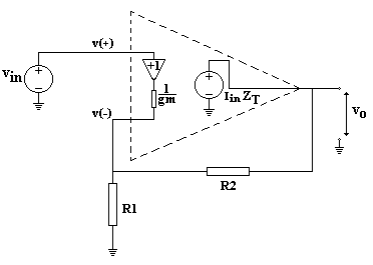
\includegraphics[scale=1]{Imagenes/CFA.png}
    \caption{CFA}
\end{figure}

\newpage
\subsection{Compensación por Adelanto}

\hspace{1mm} También denominado \textit{cero-polo} se caracteriza por generar un cero (\( f_{zx} \)) a frecuencia igual o superior al segundo polo original, corriendo de esta manera el atraso producido por este a frecuencias inferiores a la del punto crítico, mientras que el polo adjunto (\( f_{px} \)) se ubica fuera de la banda de utilización, tal que la ganancia de lazo del amplificador compensado puede expresarse como:

\bigskip
\hspace{1mm} Si \( \omega _{o2} \leq \omega _{zx} < \omega _G \) y \( \omega _{pz} \geq \geq \omega _G \)

\begin{equation}
    A_c (s) = \frac{1 + \frac{s}{\omega _{zx}}}{1 + \frac{s}{\omega _{px}}}
\end{equation}

\bigskip
\hspace{1mm} Por lo tanto.

\begin{equation}
    T'(s) = - \frac{T(0) (1 + s/\omega _{zx})}{(1 + s/ \omega _{01})(1 + s/ \omega _{o2})}
\end{equation}

\subsection{Red Paralelo Serie}

\bigskip
\hspace{1mm} Esta red esta compuesta por un capacitor y dos resistencias distribuidas de la siguiente manera.

\bigskip
\begin{figure}[!h]
    \centering
    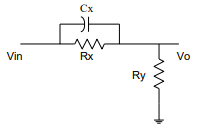
\includegraphics[scale=1]{Imagenes/Red paralelo serie.png}
    \caption{Red Paralelo Serie}
\end{figure}

\begin{equation}
    A_C (s) = \frac{V_o}{V_{in}} = \left( \frac{R}{R + R} \right) \cdot \frac{1 + sC_x R_x}{1 + sC_x (R_x // R_y)} = A(0) \cdot \frac{1 + s/\omega _{zx}}{1 + s/ \omega _{px}}
\end{equation}

\newpage
\subsection{Máxima Planicidad de Módulo}

\hspace{1mm}En aplicaciones de alta velocidad y ancho de banda, como procesamiento de señales de video y redes activas, se requieren sistemas realimentados que cumplan estrictos requisitos de ganancia, ancho de banda y distorsión de frecuencia/fase. Para optimizar el rendimiento, los amplificadores deben operar al límite de su capacidad, lo que requiere una coordinación cuidadosa entre la estabilidad del sistema y los requisitos de respuesta. Las especificaciones comunes incluyen minimizar la distorsión de frecuencia y fase en la banda de transmisión y maximizar el producto ganancia-ancho de banda. El análisis busca establecer las relaciones necesarias entre los coeficientes de la ganancia de lazo cerrado para cumplir con estos requisitos en la síntesis del sistema realimentado. Además, se considera que la ganancia del sistema en lazo cerrado presenta dos polos cuyo carácter depende de la cantidad de realimentación introducida y que la red externa al elemento activo se expresa como cociente de polinomios racionales en la variable compleja (s).

\begin{equation}
    Af(s) =  \frac{V_o}{V_{in}} = \frac{Av (s)}{1 - T(s)} = \frac{N(s)}{D(s)}
\end{equation}

\bigskip
\hspace{1mm} Dicha ecuación tiene como límites que el polinomio del denominador es como máximo de segundo grado y el polinomio del numerador no puede exceder el grado del denominador.

\hspace{1mm} Desarrollando dicha fórmula se obtiene la siguiente expresión.

\begin{equation}
    af(j \Omega) = \frac{(1 - n_2 \Omega ^2) + jn_1 \Omega}{(1 - d_2 \Omega ^2) + jd_1 \Omega}
\end{equation}

\bigskip
\hspace{1mm} Tomando módulo se deducen las relaciones que deben cumplir los coeficientes de la GLC para satisfacer la condición de máxima planicidad de módulo en la banda de transmisión.

\begin{equation}
    |af(\Omega)|^2 = \frac{(1 - n_2 \Omega ^2)^2 + (n_1 \Omega)^2}{(1 - d_2 \Omega ^2)^2 + (d_1 \Omega)^2}
\end{equation}

\begin{equation}
    |af(\Omega)|^2 = \frac{1 + a_1 \Omega ^2 + a_2 \Omega^4}{1 + b_1 \Omega ^2 + b_2 \Omega^4}
\end{equation}

\bigskip
\hspace{1mm} De la ecuación (7), función par en \( \Omega \), se infiere que la condición de invariancia del módulo con la frecuencia exige que los coeficientes de la potencias homólogas sean iguales.

\begin{equation}
    |af(\Omega)|^2 = Cte \Longrightarrow a_i = b_i \quad para \quad 0 \leq \Omega \leq \infty
\end{equation}

\bigskip
\hspace{1mm} La red que satisface esta condición se denomina pasa todo.

\bigskip
\hspace{1mm} Particularmente interesa profundizar el análisis en el caso en que N(s) sea de grado cero, por lo tanto.

\begin{equation}
    af(s) = \frac{1}{1 + \frac{s}{Q_p} + s^2}
\end{equation}

\begin{equation}
    |af(\Omega )|^2 = \frac{1}{1 + \Omega ^2 \left(\frac{1}{Q_p^2} - 2\right) + \Omega ^4}
\end{equation}

\bigskip
\hspace{1mm} Los valores de los coeficientes de esta última, en relación a la expresión general son respectivamente.

\begin{itemize}[itemsep=1pt]
    \item \( b_1 = \frac{1}{Q_p^2} - 2 \)
    \item \( b_2 = 1 \)
    \item \( a_1 = 0 \)
    \item \( a_2 = 0 \)
\end{itemize}

\bigskip
\hspace{1mm} De las cuales, la única que puede satisfacer para maxima planicidad de módulo.

\begin{equation}
    b_1 = a_1 \Longrightarrow Q_p = \frac{1}{\sqrt{2}}
\end{equation}

\bigskip
\hspace{1mm} Si esto se cumple, la expresión del módulo normalizado de la ganancia de lazo cerrado queda.

\begin{equation}
    |af(\Omega)| = \frac{1}{\sqrt{1 + \Omega ^4}}
\end{equation}

\bigskip
\hspace{1mm} La frecuencia de corte de \(3~dB\) deducida resulta.

\begin{equation}
    \frac{1}{\sqrt{1 + \Omega _H ^4}} = \frac{1}{\sqrt{2}} \Longrightarrow \Omega _H = 1 \Longrightarrow \omega _H = \omega _p
\end{equation}

\bigskip
\hspace{1mm} Es importante notar que en la banda de transmisión, la frecuencia normalizada \( \Omega )\) siempre es menor que uno, excepto en el extremo \( \Omega H \). Por lo tanto, el término de la potencia cuarta en la expresión del módulo tiene un impacto mínimo, lo que permite maximizar su planicidad.

\hspace{1mm} Para evaluar el margen de fase asociado a esta solución, es necesario conocer la ganancia de lazo involucrada.

\begin{equation}
    Avf (s) = \frac{Avf_i}{1 - \frac{1}{T(s)}} \Longrightarrow af(s) = \frac{1}{1 - \frac{1}{T(s)}} \approxeq \frac{1}{1 + \frac{s}{Q_p} + s^2}
\end{equation}

\bigskip
\hspace{1mm} De la cual se deduce la ganancia de lazo en términos normalizados.

\begin{equation}
    T(s) = - \frac{1}{\frac{s}{Q_p} + s^2} = - \frac{1}{s (s + \frac{1}{Q_p})}
\end{equation}

\bigskip
\hspace{1mm} La determinación de la frecuencia del punto crítico se obtiene a partir de la aplicación de la condición de módulo a la ecuación anterior con \( Q_p = 1/\sqrt{2} \)

\begin{equation}
    |T(\Omega G)| = 1 \Longrightarrow \Omega _G ^4 + \frac{1}{Q_p^2} \cdot \Omega_G^2 - 1 = 0 \Longrightarrow \Omega _G = 0,644
\end{equation}

\begin{equation}
    \omega _G = 0,644 \omega _p
\end{equation}

\bigskip
\hspace{1mm} Finalmente el margen de fase involucrado resulta.

\begin{equation}
    M \phi = \angle T(\Omega G) + 180 ^o = -90^o - tg^1 ( \Omega _G \cdot Q_p) + 180^o = 65,5^o 
\end{equation}





\newpage
\section{Desarrollo}
\subsection{Circuito I: VFA-VFA}
\hspace{1mm} Como se mencionó en el Objetivo, los integrados que se utilizan para el amplificador VFA es el LM324 cuyas especificaciones se detallan a continuación.

\begin{itemize}[itemsep=1pt]
    \item \(A_{d0}=100~dB\)
    \item \(F_T=1~MHz\)
    \item \(F_1=10~Hz\)
    \item \(F_2=5.06~MHz\)
\end{itemize}

\bigskip
\hspace{1mm} Seguidamente, se calculará la ganancia del circuito considerando el segundo AO como ideal. Para ello, se deberán calcular las ganancias de lazo abierto \(Ad(s)\), ganancia de lazo \(T(s)\) y ganancia de lazo cerrado \(Avf(s)\). Con todos estos datos se procederá a compensar el amplificador compuesto para lograr una máxima planicidad de módulo.

\begin{figure}[!h]
    \centering
    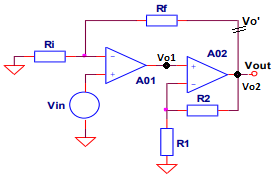
\includegraphics[scale=1.2]{Imagenes/Punto1LazoCerradoVoP.png}
    \caption{Amplificador compuesto VFA-VFA}
\end{figure}

\hspace{1mm} Por lo tanto, se comienza obteniendo la ganancia de lazo abierto. Esta misma es la relación entre la tensión de salida y la tensión de entrada.

\begin{equation}
    Av(s) = \frac{V_{out}}{V_{in}}
\end{equation}

\bigskip
\hspace{1mm} En primer lugar se buscan las variables intermedias \(V_{o1}\) y \(V_{o2}\).

\begin{equation}
    V_{o1} = Ad(s)\cdot V_{in} 
\end{equation}

\begin{equation}
     V_{o2} =V_{out}= V_{o1}\cdot (1+\frac{R_2}{R_1})
\end{equation}

\begin{equation}
    V_{o2} =V_{out}= Ad(s) \cdot V_{in} \cdot (1+\frac{R_2}{R_1})
\end{equation}

\hspace{1mm} Luego, la relación entre la salida y la entrada da como resultado la ganancia de lazo abierto.

\begin{equation}
    \boxed{
    Av(s) = Ad(s)\cdot (1+\frac{R_2}{R_1})
    }
\end{equation}

\bigskip
\hspace{1mm} Seguidamente, se calcula la ganancia de lazo.

\bigskip
\begin{equation}
    T(s) = \frac{V_{out}}{V_{out'}}|_{V_{in}=0} 
\end{equation}

\hspace{1mm} Entonces,

%aca
%aca
%aca
\begin{equation}
    V_{out}'= -\frac{R_i+R_f}{R_i}
\end{equation}

\bigskip
\hspace{1mm} Luego, \(V_{out}\) ya ha sido calculado para la ganancia de lazo abierto.

\begin{equation}
    V_{out}= V_{o1}\cdot (1+\frac{R_2}{R_1})
\end{equation}

\hspace{1mm} Por lo tanto, 

\begin{equation}
    \boxed{
      T(s) = -Ad(s)\cdot (1+\frac{R_2}{R_1})\cdot \frac{R_i}{R_i+R_f}
    }
\end{equation}

\bigskip
\hspace{1mm} Por último, la ganancia de lazo cerrado es:

\begin{equation}
    Avf(s) = \frac{Av(s)}{1-T}
\end{equation}

\begin{equation}
      Avf(s) = \frac{Ad(s)\cdot (1+\frac{R_2}{R_1})}{1+Ad(s)\cdot (1+\frac{R_2}{R_1})\cdot \frac{R_i}{R_i+R_f}}
\end{equation}

\bigskip
\hspace{1mm} Considerando la ganancia \(Ad(s)\) que tiende a ser muy grande o infinita, se simplifican los cálculos referidos a la ganancia de lazo cerrado.

\bigskip
\begin{equation}
    \boxed{
        Avf(s)=\frac{R_i+R_f}{R_i}=(1+\frac{R_f}{R_i}) 
    }
\end{equation}

\bigskip
\hspace{1mm} La consigna define que la ganancia de lazo cerrado debe ser \(Avf(s)=20~dB\). Con este dato, se puede obtener la relación entre las resistencias \(R_i\) y \(R_f\).

\begin{equation}
    Avf(s)=20~dB \hspace{3mm} \therefore \hspace{3mm} (1+\frac{R_f}{R_i})=20~dB
\end{equation}

\bigskip
\hspace{1mm} Despejando la relación de resistencias,

\bigskip
\begin{equation}
    \frac{R_f}{R_i} = 9
\end{equation}

\bigskip
\hspace{1mm} Se colocan valores arbitrarios de resistencias que cumplan con la relación recién hallada.

\begin{equation}
    \boxed{
        R_i=10~k\Omega \hspace{3mm} , R_f=90~k\Omega
    }
\end{equation}

\bigskip
\hspace{1mm} Por otro lado, con los datos de la consigna y utilizando la herramienta Matlab, se graficó el diagrama de Bode de la función de transferencia a lazo abierto del amplificador compuesto real. El mismo tiene un polo en \(10~Hz\) y otro en \(5.06~MHz\).

\begin{figure}[!h]
    \centering
    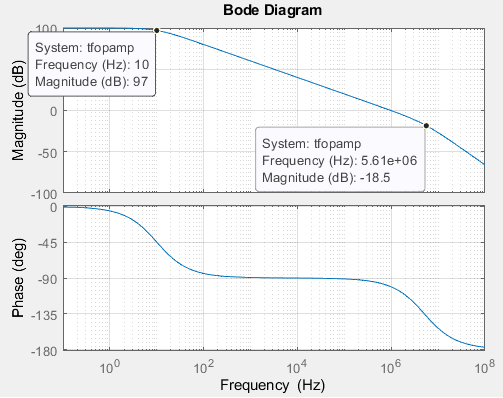
\includegraphics[scale=0.7]{Imagenes/Opamp_real_lazoabierto.png}
    \caption{Diagrama de Bode del amplificador lazo abierto}
\end{figure}

\bigskip
\hspace{1mm} Además, la consigna especifica que se debe tener máxima planicidad de módulo \(M\varphi =65°\).  A lazo cerrado se encuentra un polo en \(f_g\) el cual esta relacionado con la ganancia del amplificador AO2.


\bigskip
\hspace{1mm} Para simplificar los cálculos se consideró al amplificador AO2 como ideal, determinando a continuación la fórmula del margen de fase de la cual se despejó el polo \( 
f_g \)

\begin{equation}
    M \varphi = 180^o - arctg \left( \frac{f_g}{f_1} \right) - arctg \left( \frac{f_g}{f_2} \right) = 65,5^o
\end{equation}

\begin{equation}
    \boxed{
    f_g = 2,36~MHz
    }
\end{equation}

\bigskip
\hspace{1mm} Seguidamente, se determinó la ganancia a lazo cerrado del amplificador AO2 ideal de la siguiente manera. Considerar que la ganacia de lazo cerrado ideal fue dada en la consigna y es la siguiente \((Avfi=20~dB)\).


\begin{equation}
    Avf_{2i}=\frac{Avfi \cdot \omega_{gi}}{Ad_0 \cdot \omega_1} = 27~dB
\end{equation}

\bigskip
\hspace{1mm} Siendo \( \omega _{gi} = 2\pi f_g \)
y, \( \omega _1 \) y  \(\omega _2\) la frecuencia del primer y segundo polo respectivamente, especificada en frecuencia angular.


\bigskip
\hspace{1mm} Este valor de ganancia se utilizó para obtener la ganancia del amplificador compuesto.

\begin{equation}
    Av_{comp}=Ad0\cdot Avf_{2i}=100~dB \cdot 27~dB
\end{equation}

\begin{equation}
    \boxed{
    Av_{comp} = 127~dB
    }
\end{equation}

\begin{figure}[!h]
    \centering
    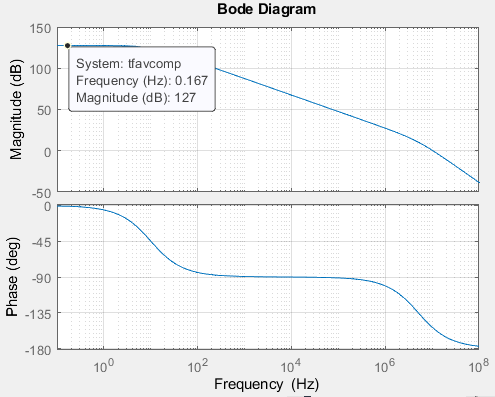
\includegraphics[scale=0.7]{Imagenes/Av_comp.png}
    \caption{Diagrama de Bode del amplificador compuesto}
\end{figure}

\bigskip
\hspace{1mm} Luego, se halló la función de transferencia de lazo cerrado del amplificador compuesto \((Avf_{comp})\). Para esto, se comenzó determinando la ganancia de ruido global \( K(global) \).

\begin{equation}
    K (global) = \frac{1}{Avf_{comp_i}} = \frac{1}{20~dB}
\end{equation}

\begin{equation}
    \boxed{
    K (global) = 0.1
    }
\end{equation}

\bigskip
\hspace{1mm} Se resolvió así la función de transferencia mencionada.

\begin{equation}
    FtAvf (comp) = \frac{Ad_0 \cdot Avf_{2i} \cdot \omega_1 \cdot \omega_2}{s^2 + s \cdot (\omega_1 + \omega_2) + (\omega_1 \cdot \omega_2 + K (global) \cdot Ad_0 \cdot Avf_{2i} \cdot \omega_1 \cdot \omega_2)}
\end{equation}

\begin{equation}
    FtAvf (comp) = \frac{4,713 \times 10^15}{s^2 + 3,179 \times 10^7 s + 4,713 \times 10^14}
\end{equation}

\bigskip
\hspace{1mm} Dicha función de transferencia se comparó con la ecuación base.

\begin{equation}
    \frac{\omega _p^2}{s^2 + s \frac{\omega _p}{Q_p } + \omega_p^2}
\end{equation}  

\bigskip
\hspace{1mm} Se igualaron las ecuaciones y se determinaron los siguientes parámetros.

\begin{equation}
    \omega _p ^2 = 4,713 \times 10^14 \Longrightarrow \omega_p =\sqrt{4,713 \times 10^14} 
\end{equation}

\begin{equation}
    \boxed{
        \omega_p = 2,17 \times 10^7
    }
\end{equation}

\bigskip
\hspace{1mm} Siendo entonces la frecuencia del polo compensado.

\begin{equation}
    f_p = \frac{\omega_p}{2\pi}
\end{equation}

\begin{equation}
    \boxed{
    f_p = 3,41\times 10^7
    }
\end{equation}

\bigskip
\hspace{1mm} Por último, se comprobó que \( Q_p \).

\begin{equation}
    Q_p = \frac{\omega_p}{3,179 \times 10^7}
\end{equation}

\begin{equation}
    \boxed{
    Q_p = 0,707
    }
\end{equation}


\begin{figure}[!h]
    \centering
    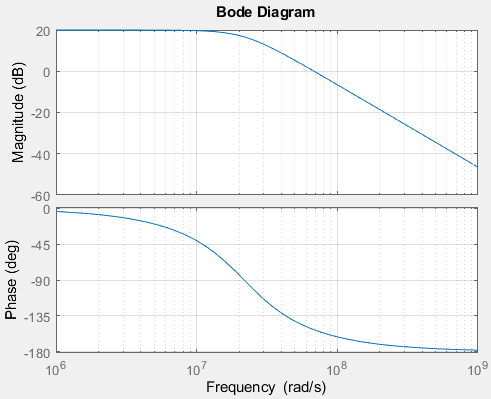
\includegraphics[scale=0.8]{Imagenes/comp_feedback.png}
    \caption{Diagrama de Bode del amplificador compuesto realimentado}
\end{figure}



\begin{figure}[!h]
    \centering
    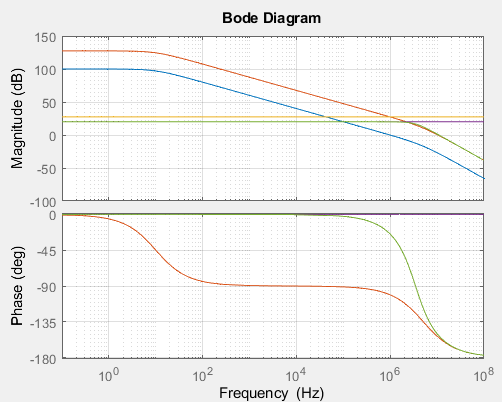
\includegraphics[scale=0.75]{Imagenes/BODE.png}
    \caption{Diagrama de Bode del amplificador VFA-VFA}
    \label{fig:foto}
        \begin{description} [itemsep=1pt, parsep=0pt, partopsep=0pt, topsep=0pt]
         \centering
         \small
         \item[Azul:]  Ganancia de AO1 a lazo abierto.
         \item[Amarillo:]  Ganancia de AO2 a lazo abierto.
         \item[Naranja:]  Ganancia del amplificador compuesto a lazo abierto.
         \item[Violeta:]  Ganancia del amplificador compuesto a lazo cerrado ideal.
         \item[Verde:]  Ganancia del amplificador compuesto a lazo cerrado real.
        \end{description}
\end{figure}

\newpage
\hspace{1mm} A través del código de Matlab, se pudo comprobar que la ganancia de lazo cerrado es igual a \(Avf_2=27.5~dB\) y, por lo tanto, la ganancia del amplificador compuesto a lazo abierto resulta ser \(127.5~dB\). Con estos valores, se puede calcular el valor del polo \(f_g\).

%Ver si encuentro la fórmula esta desps
\begin{equation}
    \frac{127.5~dB-20~dB}{log(10)-log(f_g)}=-20~dB/dec
\end{equation}

\bigskip
\hspace{1mm} Despejando \(f_g\), se obtiene:

\begin{equation}
    f_g=2.4~MHz
\end{equation}

\newpage
\subsection{Circuito II: VFA-CFA}
\hspace{1mm} Como se mencionó en el Objetivo, los integrados que se utilizan para el amplificador CFA es el LM6181 cuyas especificaciones se detallan a continuación.

\begin{itemize}[itemsep=1pt]
    \item \(R_T=2.37~M\Omega\)
    \item \(C_T=4.8~pF\)
    \item \(F_1=14~KHz\)
    \item \(F_2=82.3~MHz\)
\end{itemize}

\bigskip
\hspace{1mm} Para el desarrollo de este problema se considerará al VFA tiene el mismo comportamiento que el caso anterior y también que el polo de mayor frecuencia del CFA tiene un efecto despreciable sobre la respuesta del amplificador a lazo cerrado.

\bigskip
\hspace{1mm} Teniendo en cuenta lo mencionado, la ecuación de margen de fase para máxima planicidad se desarrolla de la siguiente manera.

\begin{equation}
    M \varphi = 180^o - arctg \left(\frac{f_g}{f_{1VFA}}\right) - arctg \left(\frac{f_g}{f_{2VFA}}\right) - arctg \left(\frac{f_g}{f_{CFA}}\right) = 65,5^o
\end{equation}

\bigskip
\hspace{1mm} Reemplazando por los valores dados.

\begin{equation}
    65,5^o = 180^o - arctg \left(\frac{2~MHz}{10~Hz}\right) - arctg \left(\frac{2~MHz}{5,06~MHz}\right) - arctg \left(\frac{2~MHz}{f_{CFA}}\right)
\end{equation}

\bigskip
\hspace{1mm} El polo \( f_{1VFA} \) se encuentra lo suficientemente alejado para no tener impacto sobre la respuesta del amplificador por lo que se lo toma como \( 90^o \)

\begin{equation}
    65,5^o = 180^o - 90^o - 21,57^o - arctg \left(\frac{2~MHz}{f_{CFA}}\right)
\end{equation}

\bigskip
\hspace{1mm} El cual resolviendo y despejando se logra.

\begin{equation}
    tg (2,93^o) = \frac{2~MHz}{f_{CFA}}
\end{equation}

\bigskip
\hspace{1mm} Finalmente la frecuencia del polo generado por el CFA es la siguiente.

\begin{equation}
    f_{CFA} = \frac{2~MHz}{tg (2,93^o)} = 39~MHz
\end{equation}

\bigskip
\hspace{1mm} Dando como resultado que para obtener una máxima planicidad la frecuencia del polo de lazo cerrado del CFA debe ser.

\begin{equation}
    \boxed{
        f_{CFA} = 39~MHz
    }
\end{equation}

\bigskip
\hspace{1mm} Obteniendo dicha frecuencia se puede calcular la resistencia \( R_2 \) partiendo de la siguiente ecuación.

\begin{equation}
    \omega _{CFA} = \frac{1}{C_T \cdot R_2}
\end{equation}

\bigskip
\hspace{1mm} De la cual se despejará \( R_2 \)

\begin{equation}
    R_2 = \frac{1}{C_T \cdot 2\pi f_{CFA}} = \frac{1}{4,8~pF \cdot 2\pi \cdot 39~MHz}
\end{equation}

\bigskip
\hspace{1mm} Dando como resultado.

\begin{equation}
    \boxed{
        R_2 = 850~\Omega
    }
\end{equation}

\bigskip
\hspace{1mm} Luego, se calculará la resistencia \( R_1 \) mediante el producto ganancia por ancho de banda.

\begin{equation}
    Avf \cdot f_g = Ado \cdot f_1 \cdot Avf_2
\end{equation}

\bigskip
\hspace{1mm} Donde \( Avf_2 \) es la ganancia ideal de lazo cerrado del CFA y se proseguirá a calcular despejando la fórmula anterior.

\begin{equation}
    Avf_2 = \frac{Avf \cdot f_g}{Ado \cdot f_1} = \frac{10 \cdot 2~MHz}{100000 \cdot 10~Hz}
\end{equation}

\bigskip
\hspace{1mm} Resultando así.

\begin{equation}
    \boxed{
    Avf_2 = 20
    }
\end{equation}

\bigskip
\hspace{1mm} Finalmente, se calculará \( R_1 \) partiendo de la siguiente ecuación.

\begin{equation}
    Avf_2 = 1 + \frac{R_2}{R_1} = 20
\end{equation}

\bigskip
\hspace{1mm} Despejando dicha ecuación.

\begin{equation}
    R_1 = \frac{R_2}{Avf_2 - 1} = \frac{850~\Omega}{20 - 1}
\end{equation}

\bigskip
\hspace{1mm} Dando como resultado.

\begin{equation}
    \boxed{
    R_1 = 44,7~\Omega
    }
\end{equation}

\bigskip
\hspace{1mm} Como se vio en el marco teórico, al trabajar en máxima planicidad de módulo la frecuencia del polo de la función de transferencia a lazo cerrado se obtiene a partir de la siguiente expresión.

\begin{equation}
    \omega _G = 0,644 \cdot \omega _p 
\end{equation}

\bigskip
\hspace{1mm} Se especifica para el diseño que el ancho de banda potencial que se requiere es de \( f_G = 2~MHz \). Por lo tanto reemplazando y despejando de la ecuación anterior \( f_p \)

\begin{equation}
    2\pi f_G = 0,644 \cdot 2\pi f_p \Longrightarrow f_p = \frac{f_G}{0,644} = \frac{2~MHz}{0,644}
\end{equation}

\bigskip
\hspace{1mm} Resultando así.

\begin{equation}
    \boxed{
    f_p = 3,1~MHz
    }
\end{equation}

\bigskip
\hspace{1mm} El ancho de banda a -3dB es igual a la frecuencia del polo a lazo cerrado, que en este caso es de 3.1 MHz, ya que esta es una condición que busca maximizar la planicidad del módulo.

\subsubsection{Simulaciones}

\hspace{1mm} Se utilizó el simulador Multisim V.14.0 para analizar el circuito final.

\begin{figure}[!h]
    \centering
    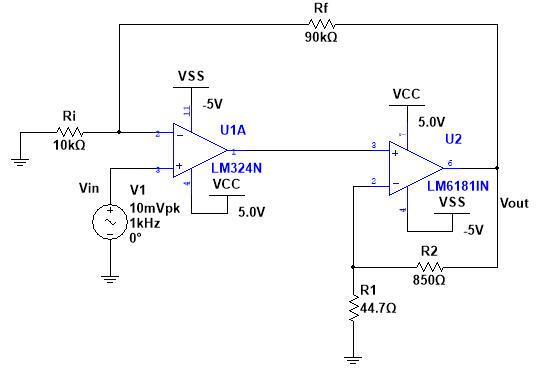
\includegraphics[width=0.6\linewidth]{Imagenes/Circuito Completo P2.png}
    \caption{Amplificador VFA-CFA}
    
\end{figure}
    
\hspace{1mm} En el cual insertó una señal sinusoidal con un valor de tensión pico de \(10~mV\) con una frecuencia de \( 1~kHz \) se obtuvieron las siguientes gráficas a la entrada (color rojo) y a la salida (color azul).

\begin{figure}[!h]
    \centering
    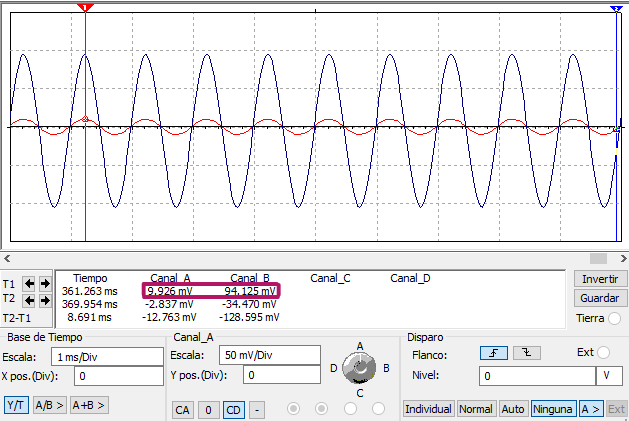
\includegraphics[width=0.7\linewidth]{Imagenes/Ganancia del Amplificador P2.png}
    \caption{Ganancia del Amplificador Compuesto.}
\end{figure}

\hspace{1mm} En donde se puede comprobar que para un valor de entrada de \( 9.926~mV \) se obtiene a la salida \( 94.125~mV \) con lo cual la ganancia obtenida es.

\begin{equation}
    G = \frac{94.125~mV}{9.926~mV}
\end{equation}

\begin{equation}
    \boxed{
    G = 9.483
    }
\end{equation}

.\hspace{1mm} En relación con la respuesta en frecuencia, se ha generado el diagrama de Bode que se muestra en la figura siguiente. En este diagrama, se observa una ganancia de \(20~dB\) y una caída de \(-3~dB\), la cual se produce a una frecuencia de \(2.0113~MHz\).

\newpage
\begin{figure}[!h]
    \centering
    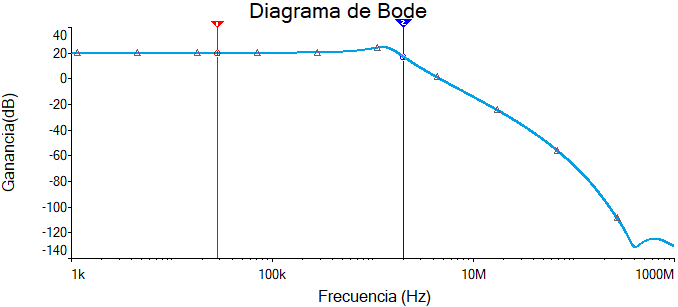
\includegraphics[width=0.7\linewidth]{Imagenes/Diagrama de Bode P2.png}
    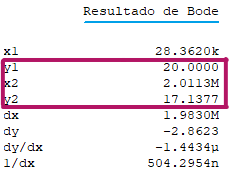
\includegraphics[width=0.25\linewidth]{Imagenes/Medidas.png}
    \caption{Diagrama de Bode.}
\end{figure}








\newpage
\subsection{Circuito III: VFA-CFA}

\hspace{1mm} Se ha diseñado una red de compensación cero-polo, como se describió anteriormente, con el propósito específico de cancelar el polo ubicado en \(5.06~MHz\) del amplificador VFA. La configuración de esta red se presenta visualmente en la siguiente figura:

\begin{figure}[!h]
    \centering
    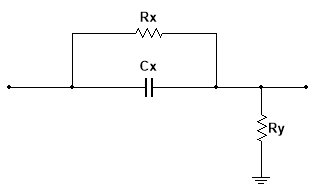
\includegraphics[width=0.5\linewidth]{Imagenes/Red de compensacion RC.png}
    \caption{Red de Compensación RC.}
\end{figure}

\hspace{1mm} En esta representación gráfica, se destacan los elementos clave de la red de compensación, incluyendo la ubicación del cero y del polo diseñados para contrarrestar el efecto del polo existente en \(5.06~MHz\).

\bigskip
\hspace{1mm} Dicha red posee la siguiente función de transferencia que la caracteriza.

\begin{equation}
    A_c(s) = \frac{R_y}{R_x + R_y} \cdot \frac{1 + sC_x R_x}{1 + sC_x (R_x // R_y)}
\end{equation}

\hspace{1mm} Donde se han definido las siguientes notaciones:

\begin{itemize}[itemsep=1pt]
    \item \(k_{comp}=\frac{R_y}{R_x + R_y}\)
    \item \( \omega_{pcomp} =  \frac{1 }{1 + sC_x (R_x // R_y)}\)
    \item \(\omega_{zcomp} = \frac{1 }{ C_xR_x}\)
\end{itemize}

\hspace{1mm} Como el cero del compensador debe cancelar el polo de frecuencia más alta del VFA, entonces.

\begin{equation}
    \omega_{zcomp} = \omega_2 = 2\pi \cdot 5.06~Mrps
\end{equation}

\hspace{1mm} El polo de compensación se encuentra una octava por encima de este cero para mantener la relación de ganancia especificada en el marco teórico. Entonces:

\begin{equation}
    \omega _{pcomp} = 2\omega _{zcomp} = 2\pi \cdot 10.12~Mrps
\end{equation}

\hspace{1mm} A partir de estos valores se pudo calcular la ganancia del compensador \(k_{comp}\)

\begin{equation}
    k_{comp} = \frac{\omega_{zcomp}}{\omega _{pcomp}} = \frac{\omega_2 = 2\pi \cdot 5.06~Mrps}{2\pi \cdot 10.12~Mrps}
    \end{equation}

\begin{equation}
    \boxed{
    k_{comp} = 0.5
    }
\end{equation}

\hspace{1mm} Por lo tanto, \(k_{comp}\) es.

\begin{equation}
    k_{comp} = \frac{R_y}{R_x + R_y} = 0.5
\end{equation}

\hspace{1mm} Se despejó para conseguir la relación entre las resistencias.

\begin{equation}
    \frac{R_y}{R_x + R_y} = \frac{1}{2} \Longrightarrow 2R_y = R_x + R_y \Longrightarrow 2 = \frac{R_x}{R_y} + 1
\end{equation}

\begin{equation}
    \boxed{
    1 = \frac{R_x}{R_y}
    }
\end{equation}

\hspace{1mm} Entonces, se consideraron valores normales de.

\begin{equation}
    \boxed{
    R_x = R_y = 1~k\Omega
    }
\end{equation}

\hspace{1mm} Con dichos valores se puede calcular el capacitor \(C_x\) despejando la fórmula de \(\omega_{zcomp}\).

\begin{equation}
    \omega_{zcomp} = \frac{1}{C_x R_x} = 2\pi \cdot 5.06~Mrps
\end{equation}

\begin{equation}
    C_x = \frac{1}{2\pi \cdot 5.06~Mrps \cdot 1~k\Omega}
\end{equation}

\begin{equation}
    \boxed{
    C_x = 31~pF
    }
\end{equation}

\hspace{1mm} Al agregar el compensador, se obtiene la siguiente función de transferencia del lazo de realimentación:

\begin{equation}
    T(s) = -A_d(s) \cdot A_c(s) \cdot A_{vf2} (s) = - \frac{kA_d(0)}{\left(1+\frac{s}{\omega_1}\right)\left(1+\frac{s}{\omega_2}\right)} \cdot k_{comp} \frac{\left(1 + \frac{s}{\omega_{zcomp}}\right)}{\left(1+\frac{s}{\omega_{pcomp}}\right)} \cdot A_{vf2}(s)
\end{equation}

\hspace{1mm} Donde:

\begin{itemize}[itemsep=1pt]
    \item k es la realimentación del VFA.
    \item \(A_d(0)\) la ganancia del VFA.
    \item \(A_{vf2}\) la función de transferencia del CFA.
    \item \( \omega_1 \) y \( \omega_2 \) los polos del VFA.
\end{itemize}

\hspace{1mm} Se observa que el valor de \(k_{comp}\) induce una atenuación en la función de transferencia, y por ende, en la ganancia. Es necesario ajustar la ganancia a lazo cerrado del CFA, teniendo en cuenta que \( k_{comp} = 0.5 \):

\begin{equation}
    A_{vf2 comp} (s) = 2A_{vf2}(s)
\end{equation}

\hspace{1mm} Esta relación garantiza que la atenuación provocada por \(k_{comp}\) se compense adecuadamente en la ganancia a lazo cerrado del Compensador de Fase Avanzada (CFA), asegurando así un rendimiento equilibrado del sistema.

\hspace{1mm} Como \(A_{vf2}\) es:

\begin{equation}
    A_{vf2} = 1 + \frac{R_2}{R_1}
\end{equation}

\hspace{1mm} Reemplazando se obtiene.

\begin{equation}
    A_{vf2 comp} (s) = 2 \left( 1 + \frac{R_2}{R_1} \right) = 2 \cdot 20
\end{equation}

\begin{equation}
    \boxed{
    A_{vf2 comp} (s) = 40
    }
\end{equation}

\hspace{1mm} Dado que el polo del Compensador de Fase Avanzada (CFA) permanece invariable con respecto al caso anterior, el valor de \(R_2\) continúa siendo \(850~\Omega\), se calculó \(R_1\) como:

\begin{equation}
    \frac{R_2}{R_1} = 40 - 1 \Longrightarrow R_1 = \frac{850~\Omega}{39}
\end{equation}

\begin{equation}
    \boxed{
    R_1 = 21.8~\Omega
    }
\end{equation}

\hspace{1mm} El margen de fase ( \(M\varphi\) ) se determina como la diferencia entre \(180^o\) y la suma de los ángulos de las funciones de ganancia a lazo cerrado del Amplificador (VFA1), la función de ganancia a lazo cerrado del Compensador de Fase Avanzada (CFA), y el ángulo de la función de transferencia del Compensador. En este caso:

\begin{equation}
    M\varphi = 180^o - arctg \left(  \frac{f_g}{f_{VFA1}}\right) - arctg \left( \frac{f_g}{f_{comp}} \right) - arctg \left( \frac{f_g}{f_{CFA}} \right)
\end{equation}

\begin{equation}
   M\varphi = 180^o - 90^o - 11.12^o - 2.93^o
\end{equation}

\begin{equation}
    \boxed{
    M\varphi = 75.9^o
    }
\end{equation}

\hspace{1mm} El ancho de banda potencial permanece inalterado en relación con el caso anterior, manteniéndose en \(2~MHz\). La frecuencia del polo de la función de transferencia a lazo cerrado se calcula aplicando el producto ganancia por ancho de banda:

\begin{equation}
    A_{vf} (0) \cdot f_g = A_{vf}(-3~dB) \cdot f_p
\end{equation}

\newpage
\hspace{1mm} Se despejó \(f_p\)

\begin{equation}
    f_p = \frac{A_{vf} (0) \cdot f_g}{A_{vf}(-3~dB)} = \frac{10.2~MHz}{7.079}
\end{equation}

\begin{equation}
    \boxed{
    f_p = 2.825~MHz
    }
\end{equation}

\hspace{1mm} Por lo tanto, el ancho de banda a \(-3~dB\) resulta igual a la frecuencia del polo, es decir, \(2.825~MHz\).

\subsubsection{Simulación}

\hspace{1mm} Se obtuvo así el circuito completo con red de compensación el cual se realizó con el simulador Multisim V.14.0.

\begin{figure}[!h]
    \centering
    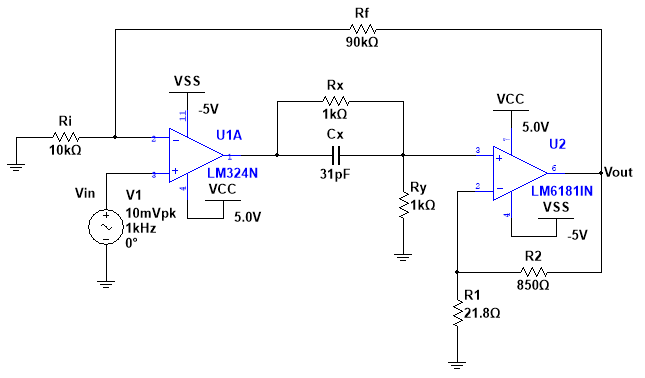
\includegraphics[width=0.7\linewidth]{Imagenes/Circuito completo compensado.png}
    \caption{Circuito Completo con Compensador.}
\end{figure}

\hspace{1mm} En el cual, como en el caso anterior, se insertó una señal sinusoidal con un valor de tensión pico de \(10~mV\) con una frecuencia de \( 1~kHz \) se obtuvieron las siguientes gráficas a la entrada (color rojo) y a la salida (color azul).

\begin{figure}[!h]
    \centering
    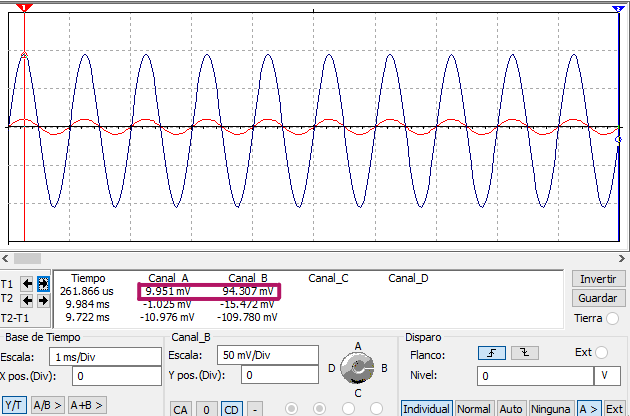
\includegraphics[width=0.7\linewidth]{Imagenes/Ganancia Amplificador Compensado.png}
    \caption{Ganancia del circuito compensado.}
\end{figure}

\hspace{1mm} En donde se puede comprobar que para un valor de entrada de \( 9.951~mV \) se obtiene a la salida \( 94.307~mV \) con lo cual la ganancia obtenida es.

\begin{equation}
    G = \frac{94.307~mV}{9.951~mV}
\end{equation}

\begin{equation}
    \boxed{
    G = 9.477
    }
\end{equation}

\newpage
.\hspace{1mm} En relación con la respuesta en frecuencia, se ha generado el diagrama de Bode que se muestra en la figura siguiente. En este diagrama, se observa una ganancia de \(20~dB\) y una caída de \(-3~dB\), la cual se produce a una frecuencia de \(2.0113~MHz\).

\begin{figure}[!h]
    \centering
    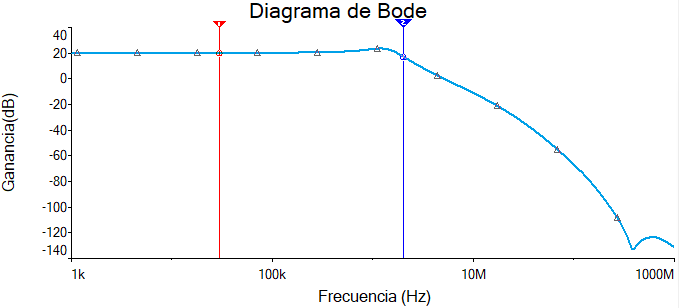
\includegraphics[width=0.7\linewidth]{Imagenes/Diagrama de Bode Compensado.png}
    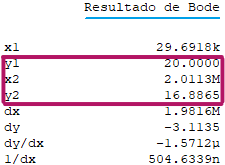
\includegraphics[width=0.25\linewidth]{Imagenes/Medidas P3.png}
    \caption{Diagrama de Bode Compensado.}
    
\end{figure}

\newpage
\section{Anexos}
\hspace{1mm} En esta sección se adjuntan los enlaces donde se encuentran los códigos y circuitos relacionados con el trabajo práctico, desarrollados en Multisim y Matlab.

\begin{itemize}
  \item Código de MATLAB: \href{https://drive.google.com/drive/u/1/folders/1tMhJg05OBsu2jBb_01hIpFwt4gK68p9m}{Enlace al código}
    \item Circuito en Multisim: \href{https://drive.google.com/drive/u/1/folders/1RTTx1D0vFVLO-MP1Zpwf79zagK8-XdSH}{Enlace al circuito}
\end{itemize}







\end{document}

